\section{Mechanism case study (model-appropriate interaction)}\label{app:mechanism}

To illustrate the model-appropriate mechanism in settings where the interaction structure is known, we examine three datasets outside the benchmark whose ground-truth targets involve multi-way feature interactions that a linear model cannot represent without explicit basis expansion. These cases are illustrative, not part of the main statistical evidence. The interaction features here are hand-constructed (all pairwise products and squares of the ordinal-coded inputs, plus all three-way products whenever the expanded matrix has fewer columns than rows), not LLM-generated formulas, so the case study illustrates the mechanism rather than the generator; KNN is not consistently helped by these exhaustive expansions (ROC-AUC changes of \(+0.040\), \(-0.071\), and \(-0.025\)), a reminder that capacity-limited does not mean uniformly helped. All numbers in this appendix are produced by one script (\texttt{scripts/run\_mechanism\_case\_study.py}) under this single protocol. The downstream models of this case study differ from the benchmark protocol: logistic regression without class weighting (up to 2,000 iterations on raw and 3,000 on expanded features), a 100-tree random forest without class weighting, and KNN with \(k = 5\), each applied after label-encoding categorical columns to ordinal codes and standardizing all columns on the full table; the metric is ROC-AUC (weighted one-vs-rest for the multiclass glass, balance-scale, and vehicle tasks) averaged over 5-fold cross-validation with 2 repeats (seed 42). We probed seven small datasets and show the three whose targets are known to involve multi-way interactions; the remaining four (glass, haberman, balance-scale, vehicle) show LR gains of \(+0.009\) to \(+0.022\) ROC-AUC with RF changes between \(-0.019\) and \(+0.023\), that is, no clear model-appropriate gap; these four are not plotted. Figure~\ref{fig:mechanism-panel} shows the LR and RF changes on the three interaction-heavy datasets.

\paragraph{Tic-tac-toe endgame (9 categorical features, 958 rows).}

The target is whether player X wins, which depends on three-in-a-row configurations, that is, on multiplicative interactions among board positions. On raw features (ordinal-coded categoricals, standardized), LR achieves ROC-AUC \(= 0.612\) while RF achieves \(0.996\). Adding pairwise and three-way interaction features raises LR to \(0.985\) (\(\Delta = +0.373\)) while RF moves to \(1.000\) (\(\Delta = +0.004\)). Before rounding, the LR gain (\(+0.3727\)) is about 98 times the RF gain (\(+0.0038\)).

\paragraph{MONK's Problem 1 (6 categorical features, 556 rows).}

The target is the known rule \((a_1 = a_2) \lor (a_5 = 1)\), whose equality term is an XOR-style interaction between two attributes. On raw features, LR achieves \(0.746\) and RF achieves \(1.000\). Interaction features raise LR to \(0.961\) (\(\Delta = +0.215\)) while RF remains at \(1.000\) (\(\Delta = 0.000\)).

\paragraph{Ionosphere (34 numeric features, 351 rows).}

Radar return classification with moderate nonlinearity. LR achieves \(0.902\) and RF achieves \(0.980\) on raw features. Pairwise products and squares (the three-way expansion would exceed the row count) raise LR to \(0.959\) (\(\Delta = +0.058\)) while RF slightly decreases to \(0.975\) (\(\Delta = -0.005\)).

These case studies demonstrate the model-appropriate mechanism concretely: when the true decision boundary involves feature interactions that LR cannot represent, explicit formula features provide large gains; when RF already captures those interactions via recursive splits, formulas are redundant or mildly harmful. They do not by themselves establish that LLM-generated formulas reliably improve LR over strong raw baselines on arbitrary tabular datasets.

\begin{figure}[htbp]
\centering
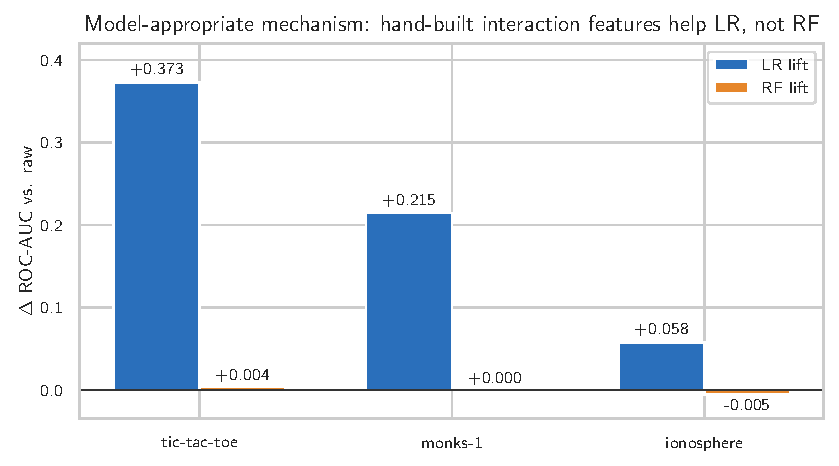
\includegraphics[width=0.8\linewidth]{figures/fig4_mechanism.pdf}
\caption{Mechanism case study on three validation datasets (not in the benchmark). Hand-constructed interaction features provide large LR gains on interaction-heavy tasks while RF remains near ceiling, illustrating why benefits can be model-appropriate rather than universal.}\label{fig:mechanism-panel}
\end{figure}


\section{Post-cutoff dataset provenance}\label{app:postcutoff-data}

Table~\ref{tab:postcutoff-data} lists the six post-cutoff tables, their Hugging Face repositories and creation dates, underlying sources and licences, sizes after preparation, and target derivations. Datasets were used as feature matrices only; free-text and most identifier columns were dropped and binary targets were derived as stated. Two retained columns are worth noting: the prediction-market table keeps a numeric market identifier and the real-estate table keeps an ordinal scrape-time code, and some generated formulas use them. Each table was fetched in June 2026. The \texttt{ImpliedData/prediction-markets} repository was public under CC BY-NC 4.0 when the table was fetched but was no longer publicly accessible on 11 October 2026, and the real-estate repository is updated continuously, so its current head differs from the table used here; the prepared feature matrices of all six tables are therefore included in the release (the prediction-market and web-tracker matrices under their original CC BY-NC 4.0 and CC BY-NC-SA 4.0 terms), so that this part of the replication remains reproducible.


\begin{table}[htbp]
\caption{Post-cutoff benchmark provenance. Sizes are rows $\times$ features after preparation (the prediction-market table is the repository's complete 40,189-row hourly candle table; its market-metadata tables were not used).}\label{tab:postcutoff-data}
\centering
\scriptsize
\begin{adjustbox}{max width=\linewidth}
\begin{tabular}{>{\raggedright\arraybackslash}p{1.9cm}>{\raggedright\arraybackslash}p{3.5cm}>{\raggedright\arraybackslash}p{3.7cm}r>{\raggedright\arraybackslash}p{1.8cm}}
\toprule
Dataset & Hugging Face repository (created) & Underlying source; licence & Size & Target \\
\midrule
clinical trials & moncefem/clinical-trials-ai-2000-2025 (2026-05-17) & ClinicalTrials.gov AI/ML trial records, 2000--2025; Apache 2.0 & \(2{,}977 \times 28\) & industry-sponsored flag \\
prediction markets & ImpliedData/prediction-markets (2026-05-17) & Polymarket/Manifold hourly candles; CC BY-NC 4.0 & \(40{,}189 \times 7\) & close above open \\
real estate & palerflavius/ro-real-estate-listings (2026-05-03) & listings scraped from imobiliare.ro; MIT & \(2{,}834 \times 7\) & price above median \\
salmonella & food-ai-nexus/salmonella-serovar-hyperspectral-spectra (2026-04-01) & \citet{papa2025rapid}, Zenodo 10.5281/zenodo.16740800; CC BY 4.0 & \(25{,}972 \times 302\) & serovar \\
web trackers & olafuraron/tracker-radar-ml (2026-03-16) & DuckDuckGo Tracker Radar with EasyPrivacy labels; CC BY-NC-SA 4.0 & \(16{,}165 \times 296\) & tracker label \\
water quality & food-ai-nexus/fecal-indicator-water-nys (2026-04-06) & PAWQ \citep{weller2020landscape,green2021integrative}, Zenodo 10.5281/zenodo.18500867; MIT & \(194 \times 94\) & E.~coli above median \\
\bottomrule
\end{tabular}
\end{adjustbox}
\end{table}

\section{Benchmark datasets}\label{app:datasets}

Table~\ref{tab:datasets} lists the 49 benchmark datasets with the OpenML dataset identifier and version that were loaded, the licence recorded on OpenML, full sizes before the 5,000-row cap, class counts, categorical-column counts as loaded, and the number of schema generators covering each dataset. Every dataset was obtained through the OpenML Python client by dataset identifier, which pins one version; the per-dataset provenance record (OpenML name, version, licence string, upload date, original source URL and citation text as published on OpenML) is released with the code as \texttt{dataset\_provenance.csv}. See Section~\ref{sec:datasets} for the three locally cached core variants and the expansion-tier selection rule.


\begin{table}[htbp]
\caption{Benchmark datasets. ``OpenML id'' and ``Ver.'' are the OpenML dataset identifier and version that were loaded (each identifier denotes one fixed version); ``Licence'' is the licence recorded on OpenML (``Public'' is an uploader assertion recorded by OpenML that no restrictive licence applies, not a formal licence; ``see source'' marks entries that name a source rather than a licence; the OpenML source description of each is in the released provenance file). Rows and features are the full table as loaded before the 5{,}000-row cap ($^{\dagger}$: local variant of the listed OpenML table, whose own listing has a different size; Section~\ref{sec:datasets}); ``Cat.'' is the number of categorical columns; ``Gen.'' is the number of schema generators with a cached linear/SVM schema for the dataset (core datasets also have tree and distance schemas from all four generators). Six core datasets (adult income, bank marketing, car evaluation, electricity, phoneme, spambase) are loaded from a local cache; for three of them (adult income, bank marketing, car evaluation) it stores the categorical columns as integer codes, which are restored to categorical columns before downstream modelling (Section~\ref{sec:protocol}); three are local variants of the listed OpenML table (Section~\ref{sec:datasets}).}\label{tab:datasets}
\centering
\scriptsize
\begin{adjustbox}{max width=\linewidth}
\begin{tabular}{llrrlrrrrr}
\toprule
Tier & Dataset & OpenML id & Ver. & Licence & Rows & Features & Classes & Cat. & Gen. \\
\midrule
core & adult\_income$^{\dagger}$ & 1590 & 2 & Public & 45{,}222 & 14 & 2 & 8 & 4 \\
core & bank\_marketing$^{\dagger}$ & 1461 & 1 & Public & 41{,}188 & 20 & 2 & 10 & 4 \\
core & blood\_transfusion & 1464 & 1 & Public & 748 & 4 & 2 & 0 & 4 \\
core & car\_evaluation & 40975 & 3 & Public & 1{,}728 & 6 & 4 & 6 & 4 \\
core & credit\_g & 31 & 1 & Public & 1{,}000 & 20 & 2 & 13 & 4 \\
core & electricity$^{\dagger}$ & 151 & 1 & Public & 38{,}474 & 7 & 2 & 0 & 4 \\
core & phoneme & 1489 & 1 & Public & 5{,}404 & 5 & 2 & 0 & 4 \\
core & pima\_diabetes & 37 & 1 & Public & 768 & 8 & 2 & 0 & 4 \\
core & qsar\_biodegradation & 1494 & 1 & Public & 1{,}055 & 41 & 2 & 0 & 4 \\
core & spambase & 44 & 1 & Public & 4{,}601 & 57 & 2 & 0 & 4 \\
\midrule
expansion & 2dplanes & 727 & 2 & Public & 40{,}768 & 10 & 2 & 0 & 3 \\
expansion & ailerons & 734 & 2 & Public & 13{,}750 & 40 & 2 & 0 & 4 \\
expansion & airlines & 42493 & 3 & Public & 26{,}969 & 7 & 2 & 5 & 4 \\
expansion & amazon\_employee\_access & 4135 & 1 & Public & 32{,}769 & 9 & 2 & 9 & 3 \\
expansion & bitcoinheist\_ransomware & 45037 & 2 & Public & 24{,}780 & 7 & 2 & 0 & 4 \\
expansion & bng\_breast\_w & 251 & 1 & Public & 39{,}366 & 9 & 2 & 0 & 4 \\
expansion & bng\_tic\_tac\_toe & 137 & 1 & Public & 39{,}366 & 9 & 2 & 9 & 2 \\
expansion & click\_prediction\_small & 1220 & 5 & Public & 39{,}948 & 9 & 2 & 0 & 4 \\
expansion & codexglue & 46682 & 1 & see source & 27{,}318 & 5 & 2 & 4 & 2 \\
expansion & coil2000\_insurance\_policies & 46916 & 1 & CC BY 4.0 & 9{,}822 & 85 & 2 & 5 & 4 \\
expansion & compass & 44162 & 3 & see source & 16{,}644 & 17 & 2 & 9 & 4 \\
expansion & customer\_churn\_classification\_nominal & 46371 & 1 & CC BY 4.0 & 35{,}000 & 24 & 2 & 0 & 4 \\
expansion & employee\_turnover\_at\_techco & 43551 & 1 & CC BY 4.0 & 34{,}452 & 9 & 2 & 0 & 4 \\
expansion & first\_order\_theorem\_proving & 1475 & 1 & Public & 6{,}118 & 51 & 6 & 0 & 4 \\
expansion & fried & 901 & 2 & Public & 40{,}768 & 10 & 2 & 0 & 4 \\
expansion & house\_16h & 821 & 2 & Public & 22{,}784 & 16 & 2 & 0 & 4 \\
expansion & house\_8l & 843 & 2 & Public & 22{,}784 & 8 & 2 & 0 & 4 \\
expansion & jungle\_chess\_2pcs\_raw\_endgame\_complete & 41027 & 1 & Public & 44{,}819 & 6 & 3 & 0 & 3 \\
expansion & kr\_vs\_kp & 3 & 1 & Public & 3{,}196 & 36 & 2 & 36 & 4 \\
expansion & law\_school\_admission\_bianry & 43890 & 2 & Public & 20{,}800 & 11 & 2 & 4 & 3 \\
expansion & led24 & 40677 & 1 & Public & 3{,}200 & 24 & 10 & 24 & 2 \\
expansion & led7 & 40678 & 1 & Public & 3{,}200 & 7 & 10 & 7 & 2 \\
expansion & loan\_approval\_status\_classification & 46526 & 1 & CC BY 4.0 & 45{,}000 & 23 & 2 & 0 & 4 \\
expansion & loan\_status & 46553 & 1 & CC BY 4.0 & 45{,}000 & 13 & 2 & 5 & 4 \\
expansion & microaggregation2 & 41671 & 1 & CC0 & 20{,}000 & 20 & 5 & 0 & 4 \\
expansion & mozilla4 & 1046 & 1 & Public & 15{,}545 & 5 & 2 & 0 & 4 \\
expansion & mushroom & 43922 & 3 & Public & 8{,}124 & 22 & 2 & 22 & 2 \\
expansion & mv & 881 & 2 & Public & 40{,}768 & 10 & 2 & 3 & 4 \\
expansion & naticusdroid & 46969 & 3 & CC BY 4.0 & 7{,}491 & 86 & 2 & 86 & 2 \\
expansion & news\_channel & 46652 & 1 & see source & 20{,}284 & 17 & 6 & 1 & 4 \\
expansion & okcupid\_stem & 45067 & 1 & Public & 26{,}677 & 13 & 3 & 11 & 1 \\
expansion & online\_shoppers & 45060 & 1 & Public & 12{,}330 & 17 & 2 & 12 & 4 \\
expansion & optdigits & 28 & 1 & Public & 5{,}620 & 64 & 10 & 0 & 3 \\
expansion & phishingwebsites & 4534 & 1 & Public & 11{,}055 & 30 & 2 & 30 & 4 \\
expansion & pol & 722 & 2 & Public & 15{,}000 & 48 & 2 & 0 & 4 \\
expansion & pricerunner & 45714 & 3 & BSD & 35{,}300 & 5 & 10 & 2 & 1 \\
expansion & splice & 46 & 1 & Public & 3{,}190 & 60 & 3 & 60 & 3 \\
expansion & taiwanese\_bankruptcy\_prediction & 46962 & 1 & CC BY 4.0 & 6{,}819 & 94 & 2 & 0 & 3 \\
expansion & volcanoes\_c1 & 1537 & 1 & Public & 28{,}626 & 3 & 5 & 0 & 4 \\
\bottomrule
\end{tabular}
\end{adjustbox}
\end{table}

\section{Core tier with all three schema families}\label{app:core-families}

The benchmark-wide analyses use the linear/SVM-family schema of each generator. On the core tier every generator also produced tree-family and distance-family schemas, giving 12 schema runs per dataset. Table~\ref{tab:core-families} reports the semantic and direct contrasts with all 12 runs averaged per dataset. The pattern matches the linear/SVM-only and benchmark-wide results: the semantic control is 10/0 for LR and KNN on ROC-AUC and 10/0 for all four models on balanced accuracy, the tree-ensemble ROC-AUC contrasts are positive but weak (RF 7/3, \(p = 0.16\); XGBoost 8/2, \(p = 0.049\)), and the direct gains are small (LR \(+0.005\), 7/3) or absent.


\begin{table}[htbp]
\caption{Core tier, all three schema families and four generators averaged per dataset ($N = 10$). Columns as in Table~\ref{tab:semantic-direct}; $p$ is the exact two-sided Wilcoxon test, whose smallest attainable value for ten datasets is 0.002.}\label{tab:core-families}
\centering
\small
\begin{adjustbox}{max width=\linewidth}
\begin{tabular}{llrrrrrrr}
\toprule
Metric & Downstream model & \(N\) & Semantic \(\Delta\) & W/L & \(p\) & Direct \(\Delta\) & W/L & \(p\) \\
\midrule
ROC-AUC & Logistic regression & 10 & +0.0115 & 10/0 & 0.002 & +0.0053 & 7/3 & 0.131 \\
ROC-AUC & KNN & 10 & +0.0632 & 10/0 & 0.002 & +0.0020 & 5/5 & 0.625 \\
ROC-AUC & Random forest & 10 & +0.0043 & 7/3 & 0.160 & -0.0011 & 4/6 & 0.625 \\
ROC-AUC & XGBoost & 10 & +0.0053 & 8/2 & 0.049 & +0.0001 & 4/6 & 0.922 \\
\midrule
Bal. accuracy & Logistic regression & 10 & +0.0135 & 10/0 & 0.002 & +0.0044 & 7/3 & 0.375 \\
Bal. accuracy & KNN & 10 & +0.0945 & 10/0 & 0.002 & +0.0219 & 6/4 & 0.105 \\
Bal. accuracy & Random forest & 10 & +0.0506 & 10/0 & 0.002 & +0.0040 & 6/4 & 0.432 \\
Bal. accuracy & XGBoost & 10 & +0.0256 & 10/0 & 0.002 & +0.0009 & 6/4 & 0.375 \\
\bottomrule
\end{tabular}
\end{adjustbox}
\end{table}

\section{Per-dataset deltas}\label{app:per-dataset}

Table~\ref{tab:per-dataset} gives the semantic-control and direct ROC-AUC deltas for every benchmark dataset and downstream model, averaged over the generators covering the dataset. Entries of \(\pm 0.000\) on mushroom, optdigits, pricerunner and similar datasets reflect raw scores at the ceiling (Appendix~\ref{app:raw-scores}).


\begin{table}[htbp]
\caption{Per-dataset ROC-AUC deltas, averaged over the generators covering each dataset (Gen.). Semantic: \texttt{raw+formula} minus \texttt{raw+permuted-formula}; direct: \texttt{raw+formula} minus \texttt{raw}.}\label{tab:per-dataset}
\centering
\scriptsize
\setlength{\tabcolsep}{3pt}
\begin{adjustbox}{max width=\linewidth}
\begin{tabular}{llrrrrrrrrr}
\toprule
& & & \multicolumn{4}{c}{Semantic $\Delta$} & \multicolumn{4}{c}{Direct $\Delta$} \\
\cmidrule(lr){4-7}\cmidrule(lr){8-11}
Tier & Dataset & Gen. & LR & KNN & RF & XGB & LR & KNN & RF & XGB \\
\midrule
core & adult\_income & 4 & +0.005 & +0.030 & -0.002 & -0.001 & +0.004 & +0.002 & +0.002 & -0.002 \\
core & bank\_marketing & 4 & +0.002 & +0.016 & -0.001 & +0.000 & +0.001 & -0.006 & +0.001 & -0.001 \\
core & blood\_transfusion & 4 & +0.026 & +0.049 & -0.036 & -0.020 & -0.000 & -0.001 & -0.004 & -0.002 \\
core & car\_evaluation & 4 & +0.008 & +0.184 & +0.006 & +0.007 & +0.003 & -0.008 & -0.000 & -0.000 \\
core & credit\_g & 4 & +0.009 & +0.091 & +0.015 & +0.019 & +0.001 & +0.033 & +0.002 & +0.000 \\
core & electricity & 4 & +0.005 & +0.089 & +0.014 & +0.013 & +0.003 & -0.001 & -0.010 & -0.003 \\
core & phoneme & 4 & +0.042 & +0.084 & +0.034 & +0.021 & +0.039 & -0.001 & +0.000 & +0.005 \\
core & pima\_diabetes & 4 & +0.014 & +0.051 & +0.013 & +0.003 & +0.003 & +0.010 & +0.006 & +0.009 \\
core & qsar\_biodegradation & 4 & +0.004 & +0.015 & +0.002 & +0.004 & -0.000 & -0.006 & -0.002 & -0.002 \\
core & spambase & 4 & +0.007 & +0.030 & +0.001 & +0.001 & +0.006 & +0.012 & -0.002 & -0.000 \\
\midrule
expansion & 2dplanes & 3 & +0.033 & +0.029 & -0.000 & -0.000 & +0.032 & +0.003 & -0.001 & -0.001 \\
expansion & ailerons & 4 & +0.000 & +0.025 & +0.007 & +0.001 & -0.000 & -0.000 & -0.000 & -0.001 \\
expansion & airlines & 4 & +0.005 & +0.024 & -0.002 & +0.009 & +0.003 & -0.020 & -0.004 & -0.005 \\
expansion & amazon\_employee\_access & 3 & +0.002 & +0.055 & +0.016 & +0.046 & +0.003 & -0.001 & +0.003 & +0.005 \\
expansion & bitcoinheist\_ransomware & 4 & +0.068 & +0.204 & +0.012 & +0.009 & +0.065 & +0.062 & -0.000 & -0.000 \\
expansion & bng\_breast\_w & 4 & +0.001 & +0.004 & -0.000 & +0.000 & +0.001 & -0.000 & -0.000 & -0.000 \\
expansion & bng\_tic\_tac\_toe & 2 & +0.008 & +0.099 & -0.000 & +0.017 & +0.007 & +0.004 & +0.004 & -0.018 \\
expansion & click\_prediction\_small & 4 & +0.034 & +0.045 & +0.006 & +0.009 & +0.022 & +0.026 & -0.006 & -0.005 \\
expansion & codexglue & 2 & +0.004 & +0.093 & +0.044 & +0.042 & -0.002 & -0.021 & +0.019 & +0.010 \\
expansion & coil2000\_insurance\_policies & 4 & +0.012 & +0.011 & +0.010 & +0.014 & +0.008 & +0.012 & +0.006 & +0.003 \\
expansion & compass & 4 & +0.008 & +0.031 & +0.039 & +0.020 & +0.006 & +0.013 & +0.007 & +0.004 \\
expansion & customer\_churn\_classification\_nominal & 4 & +0.048 & +0.043 & +0.001 & -0.001 & +0.046 & +0.024 & +0.002 & -0.001 \\
expansion & employee\_turnover\_at\_techco & 4 & +0.003 & -0.018 & +0.142 & +0.104 & -0.016 & +0.026 & +0.007 & -0.002 \\
expansion & first\_order\_theorem\_proving & 4 & +0.011 & +0.044 & -0.000 & +0.015 & +0.006 & +0.000 & -0.001 & +0.000 \\
expansion & fried & 4 & +0.064 & +0.086 & +0.024 & +0.007 & +0.063 & +0.038 & +0.017 & +0.006 \\
expansion & house\_16h & 4 & +0.027 & +0.047 & +0.001 & +0.002 & +0.025 & +0.001 & -0.002 & -0.000 \\
expansion & house\_8l & 4 & +0.023 & +0.065 & +0.002 & +0.004 & +0.022 & +0.013 & -0.002 & -0.002 \\
expansion & jungle\_chess\_2pcs\_raw\_endgame\_complete & 3 & +0.035 & +0.098 & +0.048 & +0.042 & +0.033 & -0.009 & +0.025 & +0.022 \\
expansion & kr\_vs\_kp & 4 & +0.000 & +0.054 & +0.001 & +0.000 & +0.000 & -0.012 & +0.000 & +0.000 \\
expansion & law\_school\_admission\_bianry & 3 & +0.000 & +0.022 & +0.000 & +0.000 & +0.000 & -0.014 & +0.000 & +0.000 \\
expansion & led24 & 2 & +0.002 & +0.069 & -0.004 & +0.001 & -0.000 & +0.018 & -0.003 & +0.002 \\
expansion & led7 & 2 & +0.001 & +0.036 & -0.004 & +0.006 & -0.000 & -0.004 & -0.000 & -0.003 \\
expansion & loan\_approval\_status\_classification & 4 & +0.004 & +0.017 & +0.001 & +0.001 & +0.003 & +0.010 & -0.002 & -0.001 \\
expansion & loan\_status & 4 & +0.003 & +0.052 & +0.002 & +0.001 & +0.002 & +0.006 & -0.001 & -0.001 \\
expansion & microaggregation2 & 4 & +0.020 & +0.040 & -0.001 & +0.014 & +0.013 & -0.001 & -0.005 & +0.002 \\
expansion & mozilla4 & 4 & +0.031 & +0.139 & +0.017 & +0.012 & +0.026 & +0.015 & -0.001 & +0.002 \\
expansion & mushroom & 2 & +0.000 & +0.000 & +0.000 & +0.000 & +0.000 & -0.000 & +0.000 & +0.000 \\
expansion & mv & 4 & +0.000 & +0.023 & +0.001 & +0.000 & +0.000 & +0.001 & +0.000 & -0.000 \\
expansion & naticusdroid & 2 & +0.000 & +0.005 & -0.002 & +0.001 & -0.000 & -0.003 & -0.000 & -0.000 \\
expansion & news\_channel & 4 & +0.013 & +0.054 & +0.016 & +0.017 & +0.007 & +0.013 & +0.004 & +0.006 \\
expansion & okcupid\_stem & 1 & -0.000 & +0.066 & -0.000 & +0.002 & -0.000 & +0.009 & +0.002 & -0.001 \\
expansion & online\_shoppers & 4 & +0.027 & +0.117 & +0.009 & -0.001 & +0.024 & +0.055 & +0.007 & -0.003 \\
expansion & optdigits & 3 & +0.000 & +0.000 & +0.000 & +0.000 & +0.000 & +0.000 & -0.000 & +0.000 \\
expansion & phishingwebsites & 4 & +0.000 & +0.018 & -0.000 & +0.003 & -0.000 & -0.001 & -0.000 & -0.000 \\
expansion & pol & 4 & +0.037 & +0.025 & +0.002 & +0.001 & +0.037 & +0.003 & +0.000 & +0.000 \\
expansion & pricerunner & 1 & +0.000 & +0.050 & +0.000 & +0.000 & -0.000 & -0.000 & -0.000 & +0.000 \\
expansion & splice & 3 & +0.000 & +0.025 & -0.000 & -0.000 & +0.000 & +0.018 & -0.001 & -0.000 \\
expansion & taiwanese\_bankruptcy\_prediction & 3 & +0.001 & +0.024 & -0.004 & +0.003 & -0.001 & +0.004 & -0.000 & +0.001 \\
expansion & volcanoes\_c1 & 4 & +0.038 & +0.035 & -0.008 & -0.027 & -0.024 & +0.003 & +0.022 & -0.025 \\
\bottomrule
\end{tabular}
\end{adjustbox}
\end{table}

\section{Raw baseline scores}\label{app:raw-scores}

Table~\ref{tab:raw-scores} reports the raw-feature ROC-AUC of each downstream model on each benchmark dataset. Nine datasets (bng\_breast\_w, car evaluation, kr\_vs\_kp, law school admission, mushroom, mv, optdigits, pol, pricerunner) have raw XGBoost at or above 0.995, so the absence of a tree-ensemble gain there is a ceiling effect; the datasets carrying the LR direct gain are those where raw LR trails the tree ensembles the most (Section~\ref{sec:direct}).


\begin{table}[htbp]
\caption{Raw-feature ROC-AUC per dataset and downstream model (generator-averaged evaluation split; the raw matrix is shared across generators).}\label{tab:raw-scores}
\centering
\scriptsize
\begin{adjustbox}{max width=\linewidth}
\begin{tabular}{llrrrr}
\toprule
Tier & Dataset & LR & KNN & RF & XGB \\
\midrule
core & adult\_income & 0.912 & 0.895 & 0.910 & 0.923 \\
core & bank\_marketing & 0.937 & 0.897 & 0.936 & 0.941 \\
core & blood\_transfusion & 0.764 & 0.730 & 0.702 & 0.703 \\
core & car\_evaluation & 0.981 & 0.971 & 0.997 & 0.998 \\
core & credit\_g & 0.793 & 0.736 & 0.800 & 0.793 \\
core & electricity & 0.819 & 0.838 & 0.888 & 0.891 \\
core & phoneme & 0.805 & 0.914 & 0.953 & 0.936 \\
core & pima\_diabetes & 0.823 & 0.795 & 0.820 & 0.797 \\
core & qsar\_biodegradation & 0.914 & 0.905 & 0.926 & 0.925 \\
core & spambase & 0.972 & 0.955 & 0.986 & 0.989 \\
\midrule
expansion & 2dplanes & 0.922 & 0.970 & 0.981 & 0.985 \\
expansion & ailerons & 0.952 & 0.913 & 0.940 & 0.953 \\
expansion & airlines & 0.625 & 0.624 & 0.645 & 0.654 \\
expansion & amazon\_employee\_access & 0.747 & 0.666 & 0.762 & 0.703 \\
expansion & bitcoinheist\_ransomware & 0.704 & 0.806 & 0.913 & 0.915 \\
expansion & bng\_breast\_w & 0.997 & 0.994 & 0.997 & 0.998 \\
expansion & bng\_tic\_tac\_toe & 0.755 & 0.813 & 0.813 & 0.859 \\
expansion & click\_prediction\_small & 0.620 & 0.581 & 0.646 & 0.655 \\
expansion & codexglue & 0.796 & 0.647 & 0.694 & 0.673 \\
expansion & coil2000\_insurance\_policies & 0.688 & 0.636 & 0.724 & 0.737 \\
expansion & compass & 0.733 & 0.711 & 0.789 & 0.761 \\
expansion & customer\_churn\_classification\_nominal & 0.809 & 0.807 & 0.874 & 0.875 \\
expansion & employee\_turnover\_at\_techco & 0.660 & 0.527 & 0.684 & 0.674 \\
expansion & first\_order\_theorem\_proving & 0.703 & 0.768 & 0.823 & 0.823 \\
expansion & fried & 0.915 & 0.930 & 0.968 & 0.980 \\
expansion & house\_16h & 0.888 & 0.907 & 0.940 & 0.944 \\
expansion & house\_8l & 0.893 & 0.909 & 0.941 & 0.944 \\
expansion & jungle\_chess\_2pcs\_raw\_endgame\_complete & 0.809 & 0.900 & 0.929 & 0.948 \\
expansion & kr\_vs\_kp & 0.993 & 0.982 & 0.999 & 0.999 \\
expansion & law\_school\_admission\_bianry & 1.000 & 0.983 & 1.000 & 1.000 \\
expansion & led24 & 0.950 & 0.915 & 0.949 & 0.940 \\
expansion & led7 & 0.956 & 0.934 & 0.941 & 0.954 \\
expansion & loan\_approval\_status\_classification & 0.954 & 0.934 & 0.963 & 0.967 \\
expansion & loan\_status & 0.951 & 0.937 & 0.963 & 0.967 \\
expansion & microaggregation2 & 0.700 & 0.667 & 0.747 & 0.767 \\
expansion & mozilla4 & 0.873 & 0.902 & 0.968 & 0.966 \\
expansion & mushroom & 1.000 & 1.000 & 1.000 & 1.000 \\
expansion & mv & 0.999 & 0.987 & 0.999 & 1.000 \\
expansion & naticusdroid & 0.978 & 0.974 & 0.976 & 0.982 \\
expansion & news\_channel & 0.746 & 0.702 & 0.751 & 0.763 \\
expansion & okcupid\_stem & 0.779 & 0.736 & 0.779 & 0.793 \\
expansion & online\_shoppers & 0.885 & 0.845 & 0.908 & 0.922 \\
expansion & optdigits & 0.999 & 0.998 & 1.000 & 0.999 \\
expansion & phishingwebsites & 0.985 & 0.984 & 0.991 & 0.992 \\
expansion & pol & 0.940 & 0.987 & 0.997 & 0.998 \\
expansion & pricerunner & 1.000 & 1.000 & 1.000 & 1.000 \\
expansion & splice & 0.991 & 0.971 & 0.994 & 0.994 \\
expansion & taiwanese\_bankruptcy\_prediction & 0.910 & 0.857 & 0.927 & 0.941 \\
expansion & volcanoes\_c1 & 0.792 & 0.762 & 0.830 & 0.882 \\
\bottomrule
\end{tabular}
\end{adjustbox}
\end{table}

\section{Second judgment model}\label{app:judgment-v4pro}

As a robustness check on the judgment null of Section~\ref{sec:per-row-judgments-add-no-reliable-value-beyond-formulas}, the same incremental contrast was computed for the 93 core schema runs whose per-row judgments were produced by DeepSeek-V4-Pro (coverage 3 to 12 of the 12 cells per dataset; the remaining 15 V4-Pro runs were not completed and 12 cells have no V4-Pro judgments). Table~\ref{tab:judgment-v4pro} shows the same picture as the DeepSeek-Reasoner runs: every ROC-AUC increment is within \(\pm 0.002\) of zero (LR \(-0.0005\), 1/9; KNN \(-0.0019\), 4/6; RF \(+0.0020\), 4/6; XGBoost \(+0.0002\), 2/8) and every balanced-accuracy increment is negative with three or four wins out of ten; no cell reaches significance. These runs are excluded from the main analysis only so that every judgment cell in Table~\ref{tab:judgment} shares one judgment model; they are produced by \texttt{scripts/expansion/judgment\_second\_model.py} from the stored results.

\begin{table}[htbp]
\caption{Second judgment model: incremental effect of DeepSeek-V4-Pro per-row judgment features beyond deterministic formulas on the ten core datasets (93 completed schema runs; coverage per dataset 3 to 12 of 12 cells, averaged per dataset before testing). Columns as in Table~\ref{tab:judgment}; $p$ is the exact two-sided Wilcoxon test over datasets.}\label{tab:judgment-v4pro}
\centering
\small
\begin{tabular}{llrrrrr}
\toprule
Metric & Downstream model & \(N\) & Mean \(\Delta\) & W/L/T & Cliff's \(\delta\) & \(p\) \\
\midrule
ROC-AUC & Logistic regression & 10 & -0.0005 & 1/9/0 & -0.80 & 0.0645 \\
ROC-AUC & KNN & 10 & -0.0019 & 4/6/0 & -0.20 & 0.3223 \\
ROC-AUC & Random forest & 10 & +0.0020 & 4/6/0 & -0.20 & 0.9219 \\
ROC-AUC & XGBoost & 10 & +0.0002 & 2/8/0 & -0.60 & 0.2754 \\
\midrule
Bal. accuracy & Logistic regression & 10 & -0.0004 & 3/7/0 & -0.40 & 0.3750 \\
Bal. accuracy & KNN & 10 & -0.0032 & 3/7/0 & -0.40 & 0.1602 \\
Bal. accuracy & Random forest & 10 & -0.0009 & 3/7/0 & -0.40 & 0.3223 \\
Bal. accuracy & XGBoost & 10 & -0.0023 & 4/6/0 & -0.20 & 0.1934 \\
\bottomrule
\end{tabular}
\end{table}


\section{Protocol details}\label{app:protocol-details}

\subsection*{Protocol details}

\paragraph{Schema summary and schema sizes.}

The summary also carries the dataset's registry name (for example \texttt{adult\_income}), the target column name, the number of design rows and, for categorical columns, the number of distinct values and the count of each of the ten most frequent values; Section~\ref{sec:anon} replaces the first two. The generator is asked for a fixed schema of 12 features. All 120 core schemas and 125 of the 131 expansion schemas have exactly 12 features; the six exceptions are truncated responses described in Section~\ref{sec:scale-of-evaluation}. The schemas contain 10.1 deterministic formula features per schema on average over the 120 core schemas (10.2 for their linear/SVM family) and 9.7 on the expansion datasets, range 1 to 11; the remainder are per-row judgment specifications (one to five on the core tier, zero to nine on the expansion tier, where they are never materialized; Section~\ref{sec:judgment}).

\paragraph{Judgment generation.}

Judgments were produced for the ten core datasets by DeepSeek-Reasoner in batches of 25 rows per call; all 12 schema runs per core dataset have a judgment matrix, so the judgment comparison covers the full core grid. A second set of judgment runs with DeepSeek-V4-Pro (93 completed matrices and 15 partially filled runs) is excluded from the main analysis so that every judgment cell shares one judgment model; Appendix~\ref{app:judgment-v4pro} reports the same contrast on the completed runs. No judgments were generated for the expansion datasets.

\paragraph{Declared value range.}

The declared range of a feature is the \texttt{value\_range} interval the generator returns for it in the schema; the materialized formula column and the parsed judgment values are clipped to this interval, and the random control draws uniform values over the same interval (the range is immaterial after standardization and for tree models).

\paragraph{Random-expression templates and sampling.}

The expressions are sampled from the vocabulary the LLM formulas use (logarithms, \(z\)-scores, min--max scaling, squares and square roots, ratios, products, sums, differences, shares, threshold and two-way indicators, three-way buckets, and category indicators), using only the design-split column statistics the generators received (means, standard deviations, minima, maxima, and the most frequent categories). An expression that is constant or undefined on the design split is redrawn, and the declared value range is the design-split range. Materialization, range clipping, cross-validation folds, downstream models, and column permutation are identical to those applied to the LLM formulas. Five random schemas are drawn per cell, seeded by the cell and the draw index, and every reported random-expression score is the mean over the five draws.

\paragraph{Categorical encoding of the cached core datasets.}

The local cache of adult income, bank marketing, and car evaluation stores their categorical columns as 8-bit integer codes, and the schema generators received these columns summarized as numeric (mean, standard deviation, minimum, maximum), so their formulas reference the codes. The evaluation keeps the formulas exactly as written, computing them on the codes, but restores the columns to categoricals before downstream modelling, so the raw block is mode-imputed and one-hot encoded as for every other dataset; the random, permuted, and judgment matrices of these runs share the same rows and encoding. An earlier version of this evaluation passed the codes to the downstream models as ordinal integers, which weakened the raw LR and KNN baselines on the three datasets and inflated the formula gains there, most visibly on car evaluation; every number in this paper uses the one-hot encoding.

\paragraph{Row cap and design splits for schema generation.}

On the core tier the 5,000-row cap was applied to adult income, bank marketing and electricity, while phoneme, with 5,404 rows, was evaluated uncapped. The schema generators for the core datasets received the column-level summary of a 20--30\% design split of the full, uncapped dataset (for nine Claude Sonnet 4.6 cells on blood transfusion, credit-g, pima diabetes, and QSAR biodegradation, of the full dataset); because the 5,000-row cap nests inside that split, the summary statistics for adult income, bank marketing, and electricity also cover the rows later used for evaluation. Only distributional statistics and the class balance are exposed, never row-level labels, and Section~\ref{sec:leakage} checks that this overlap does not inflate the effects. The expansion schemas were generated from the column-level summary of a stratified 30\% design split (seed 42) of the full, uncapped dataset; the 5,000-row evaluation cap is drawn afterwards, so for the 35 expansion datasets with more than 5,000 rows the summary statistics also cover rows that later serve as evaluation rows, exactly as for the three capped core datasets, and only for the four expansion datasets with at most 5,000 rows (kr\_vs\_kp, led7, led24, splice) are the design and evaluation rows disjoint. As on the core tier, only distributional statistics and the class balance were exposed, and the check of Section~\ref{sec:leakage} bounds the effect of this overlap.

\paragraph{Multiplicity across tables.}

As a global check, Benjamini-Hochberg over the 48 dataset-level tests of Tables~\ref{tab:semantic-direct} and~\ref{tab:random-expression} leaves every cell reported as significant below \(q = 0.05\) (largest 0.019); Holm over all 48 retains every semantic effect (RF at 0.044), the LR direct gain, the LR, KNN, and RF LLM-minus-random-expression contrasts, and all excess-semantic cells, but not the KNN direct gain (either metric), the balanced-accuracy RF direct gain, or the ROC-AUC random-expression-versus-raw cells for LR and XGBoost, which we therefore describe as fragile. Holm over the 16 per-generator semantic cells of Table~\ref{tab:generators} leaves all of them below 0.05 (largest 0.026).


\section{Schema and run provenance}\label{app:provenance}

\subsection*{Schema and run provenance}

\paragraph{Expansion tier composition and coverage.}

The 39 datasets range from 3,190 to 45,000 rows and from 3 to 94 raw features, 11 are multiclass (3 to 10 classes), and 20 contain categorical columns. Each expansion dataset has the linear/SVM-family schema of every generator that produced one: 24 of the 39 are covered by all four generators, seven by three (2dplanes, amazon employee access, jungle chess, law school admission, optdigits, splice, Taiwanese bankruptcy), six by two (bng\_tic\_tac\_toe, codexglue, led7, led24, mushroom, naticusdroid), and two by one (okcupid\_stem, pricerunner). The 131 expansion-tier runs come from 48, 44, 40 and 39 datasets covered by GPT-5.5 Pro, Gemini 3.1 Pro Preview, Claude Opus 4.7 and Claude Sonnet 4.6 respectively, counting the core datasets. For 13 schema cells on seven datasets whose column names are not valid Python identifiers (for GPT-5.5 Pro: amazon employee access, bng\_tic\_tac\_toe, led7, led24, mushroom, naticusdroid, phishingwebsites; for Gemini: the same set without amazon employee access), the generator saw column names sanitized to valid identifiers and the same renaming is applied to the evaluation rows before the formulas are materialized.

\paragraph{Response accounting.}

The schema cache holds 174 raw generator responses for the core datasets, 150 of them from the four benchmark generators, of which 16 failed JSON parsing or formula validation (Claude Sonnet 4.6: 10, Gemini 3.1 Pro Preview: 4, Claude Opus 4.7: 2, GPT-5.5 Pro: 0); the remaining 24 responses (7 failures) come from two earlier Gemini versions tried in a May 2026 pilot on four core datasets and are not part of the benchmark. Twelve Claude Sonnet 4.6 cells on those four datasets have two or three valid cached schemas, generated from different design-split summaries on 9 May and 30 May 2026; for these cells the pipeline used the first file returned by a directory listing, a rule fixed before any evaluation that never consults a result, and all candidate files are released. Every other cell has exactly one valid schema. The expansion schemas are cached generator responses from 3 June 2026 under the same prompt, feature budget, and design-split summary protocol (the prompt hashes of the cached files are reproduced by the current prompt builder); they were evaluated offline on 8 September 2026 without any further LLM call. Six expansion responses (Gemini 3.1 Pro Preview on splice, kr\_vs\_kp, and phishingwebsites; GPT-5.5 Pro on mushroom, phishingwebsites, and naticusdroid) were truncated before the JSON closed; the complete feature objects that could be decoded (1 to 9 formula features and no judgment specification) were kept as the schema, which accounts for all but two of the runs with fewer than five formula columns, and their formulas pass the same validator at materialization.

\paragraph{Judgment-feature audit.}

Per-row judgment features are evaluated as an incremental addition on all 120 core runs. A judgment-feature audit of the 226 stored judgment features across these runs (\texttt{scripts/audit\_judgment\_signal.py}) found no missing values: the median feature takes 109 distinct values (quartiles 16 to 402), three features are near-constant (one value covering at least 80\% of rows), 14 have more than half of their values at a declared bound, and the judgment columns alone reach ROC-AUC 0.66 with logistic regression (median 0.65, range 0.47 to 0.83 over the 120 runs; above 0.60 in 93 runs), so they encode row-level signal. A looser boundary warning, which fires whenever a single value equals a declared endpoint, is raised for 217 of the 226 features but does not indicate degenerate outputs.

\paragraph{Constant-column scan.}

Across the 251 runs no materialized formula column is entirely missing; 25 columns in 15 runs are constant on the evaluation rows (for example a monetary-to-frequency ratio that is exactly 250 on blood transfusion, or sums of a permutation-coded block on microaggregation2), and five runs materialize fewer than five non-constant formula columns (Gemini on codexglue and splice; GPT-5.5 Pro on mushroom, naticusdroid and pricerunner). All runs are kept.

\paragraph{Leakage-equivalence check.}

Because the core schemas were generated from summaries of uncapped design splits (Section~\ref{sec:protocol}), a leakage-equivalence check compares the same Claude Sonnet 4.6 and Gemini 3.1 Pro schemas evaluated prospectively (the 80\% complement of a 20\% design split, seed 42, with no row cap, hence larger evaluation sets; for the 40 of the 60 Claude Sonnet 4.6 and Gemini 3.1 Pro schemas that were generated from that 20\% split the evaluation rows are disjoint from the summarized rows, while 11 schemas were generated from a 30\% split and 9 from the full dataset) against the cached core evaluation, on the 54 overlapping cells (9 datasets, LR/RF/KNN, two metrics). The mean absolute difference in cached-versus-prospective deltas is 0.0050, with signed cached-minus-prospective difference \(+0.0023\) (largest for KNN balanced accuracy, \(+0.014\)). The two evaluation modes therefore look broadly similar at this aggregation level; the check bounds the effect of the summary-statistics overlap on the raw-to-formula deltas rather than comparing two schema-generation regimes. The cached side averages every stored run of a dataset, including the DeepSeek-V4-Pro duplicates that re-evaluate the same formula matrices.

\paragraph{Generator settings and compute.}

Schema generation sent temperature 0 to Gemini, Claude Sonnet, and DeepSeek, omitted it for the GPT-5.5 Pro and Claude Opus 4.7 reasoning endpoints, requested reasoning effort high from GPT-5.5 Pro, set no extended-thinking parameter for the other generators (Gemini 3.1 Pro Preview reasons at its API default), used JSON output mode where available (OpenAI, Gemini, DeepSeek), and used output budgets of 16,384 tokens for GPT-5.5 Pro and 8,192 tokens otherwise; the \texttt{reasoning: max\_available} entries in the released model configuration are not transmitted to the Anthropic or Gemini APIs. Table~\ref{tab:models} lists the API identifiers, endpoints, settings, and query dates; the stored responses record the alias passed to the API, token counts, and text, but not the provider's resolved snapshot identifier. All downstream evaluations ran on one Apple Silicon workstation (10 cores, 24 GB): the four-generator expansion tier took about three hours, the classical baselines on the expansion datasets about three hours, and the random-expression control about 25 minutes on five worker processes. One schema is drawn per generator, family, and dataset cell and cached by prompt hash, so the reported means carry no schema-sampling variance.

\begin{table}[tbp]
\caption{Language-model endpoints, settings, and query windows. Identifiers are the strings passed to the provider APIs (\texttt{configs/llm\_models.yaml}); dates are those of the cached responses. OpenAI documents \texttt{gpt-5.5-pro-2026-04-23} as the snapshot behind the \texttt{gpt-5.5-pro} alias; the other aliases are not version-pinned by their providers.}\label{tab:models}
\centering
\scriptsize
\setlength{\tabcolsep}{4pt}
\begin{tabular}{>{\raggedright\arraybackslash}p{1.3cm}>{\raggedright\arraybackslash}p{1.6cm}>{\raggedright\arraybackslash}p{2.8cm}>{\raggedright\arraybackslash}p{2.0cm}>{\raggedright\arraybackslash}p{2.8cm}>{\raggedright\arraybackslash}p{3.0cm}}
\toprule
Role & Name in text & API identifier & Endpoint & Settings & Queried \\
\midrule
Schema generator & GPT-5.5 Pro & \texttt{gpt-5.5-pro} & OpenAI Responses API & reasoning effort high; no temperature; 16,384 output tokens; JSON mode & core 1 June 2026; expansion 3 June; post-cutoff 8 June (one retry 21 June); anonymized 21 June \\
Schema generator & Gemini 3.1 Pro Preview & \texttt{gemini-3.1-pro-}\allowbreak\texttt{preview} & Google Generative Language API & temperature 0; 8,192 tokens; JSON mode; default thinking & core 31 May to 1 June 2026; expansion 3 June; post-cutoff 8 June \\
Schema generator & Claude Opus 4.7 & \texttt{claude-opus-4-7} & Anthropic Messages API & no temperature; 8,192 tokens & core 31 May to 1 June 2026; expansion 3 June \\
Schema generator & Claude Sonnet 4.6 & \texttt{claude-sonnet-4-6} & Anthropic Messages API & temperature 0; 8,192 tokens & core 9 May and 30 May to 1 June 2026; expansion 3 June \\
Judgment filler & DeepSeek-Reasoner & \texttt{deepseek-}\allowbreak\texttt{reasoner} & DeepSeek chat completions & temperature 0; JSON mode; 25 rows per call & 1 to 2 June 2026 \\
Judgment filler (Appendix~\ref{app:judgment-v4pro}) & DeepSeek-V4-Pro & \texttt{deepseek-v4-pro} & DeepSeek chat completions & temperature 0; JSON mode; 25 rows per call & 1 to 3 June 2026 \\
\bottomrule
\end{tabular}
\end{table}

\paragraph{Benchmark table licences and maintenance.}

The derived artifacts released under CC BY 4.0 are the schemas, responses, judgment outputs, scores, and statistics; the stored feature matrices are regenerable from the cached schemas. The OpenML benchmark tables are fetched by dataset identifier, which pins one version; the release redistributes only the six locally cached core tables (the three variants of Section~\ref{sec:datasets} and verbatim copies of car evaluation, phoneme, and spambase, all recorded as public on OpenML), the prepared post-cutoff tables of Table~\ref{tab:postcutoff-data} under their own licences (included because one repository is no longer public and another is updated continuously; Appendix~\ref{app:postcutoff-data}), and, inside every stored feature matrix, the raw evaluation-split columns of the dataset concerned. The authors maintain the repository, accept issues and corrections, and record changes in a changelog; a datasheet-style description of the benchmark (composition, preparation, intended uses, licences, hosting, and maintenance) accompanies the supplementary material.


\section{Additional tables and figures}\label{app:extra-tables}

\subsection*{Random-feature and permuted-formula controls}

Table~\ref{tab:random-controls} shows the random-feature controls.


\begin{table}[tbp]
\caption{Random-feature and permuted-formula controls versus raw features on all 49 datasets (ROC-AUC, generator-averaged). Every count-matched control degrades every model; W/L counts datasets on which the control beats raw.}\label{tab:random-controls}
\centering
\small
\begin{adjustbox}{max width=\linewidth}
\begin{tabular}{lrrrrrrr}
\toprule
Downstream model & \(N\) & Random-formula \(-\) raw & W/L & Random-all \(-\) raw & W/L & Permuted \(-\) raw & W/L \\
\midrule
Logistic regression & 49 & -0.0038 & 4/44 & -0.0065 & 0/48 & -0.0044 & 3/45 \\
KNN & 49 & -0.0474 & 2/47 & -0.0585 & 2/47 & -0.0443 & 2/47 \\
Random forest & 49 & -0.0083 & 9/38 & -0.0110 & 10/37 & -0.0067 & 11/36 \\
XGBoost & 49 & -0.0127 & 3/43 & -0.0148 & 3/44 & -0.0085 & 5/41 \\
\bottomrule
\end{tabular}
\end{adjustbox}
\end{table}

\subsection*{Where the semantic effect is largest}

The largest effects come from datasets with interaction-heavy or ratio-friendly structure (bitcoinheist ransomware, fried, customer churn, phoneme, volcanoes and pol for LR; bitcoinheist, car evaluation, mozilla4 and online shoppers for KNN), and the effect vanishes for every model only where every raw model is already at the ceiling (mushroom and optdigits, where all four raw models are at or above ROC-AUC 0.998; pricerunner is equally saturated but keeps a KNN effect; Appendix~\ref{app:per-dataset}).

\subsection*{Critical-difference diagrams}

Figure~\ref{fig:cd} shows the critical-difference diagrams summarized in Section~\ref{sec:model-appropriate-interaction}. Under the standard Demšar convention (lower average rank is better), ranks are averaged over the 49 datasets among the raw, formula, permuted-formula, random-formula, and random-all variants, and the critical difference is from the Nemenyi post-hoc test at \(\alpha = 0.05\) with \(k = 5\) treatments and \(N = 49\) (CD \(= 0.87\)). For LR, \texttt{raw+formula} attains the best average rank (1.37) ahead of raw features (1.90), with the permuted and random controls more than one CD behind (3.63 to 4.43); the formula-versus-raw gap is itself within one CD. For XGBoost raw features rank first (1.70) with \texttt{raw+formula} second (2.03) and the three controls again more than one CD behind. KNN mirrors LR (formula 1.47, raw 1.71) and RF mirrors XGBoost (raw 2.12, formula 2.39). For LR, KNN and XGBoost the aligned formula matrix is separated from its permuted copy by more than the critical difference; for RF the gap (2.90 versus 2.39) is within it, consistent with RF's small semantic effect.

\begin{figure}[tbp]
\centering
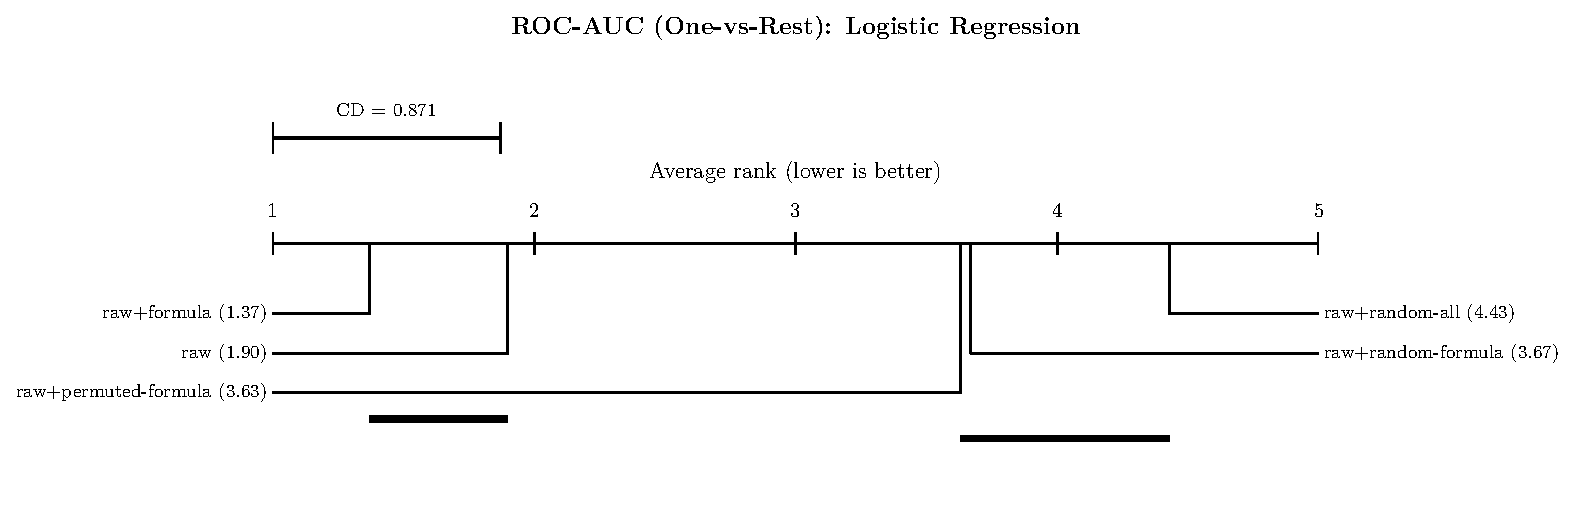
\includegraphics[width=0.85\linewidth]{figures/fig3a_cd_lr.pdf}\\[4pt]
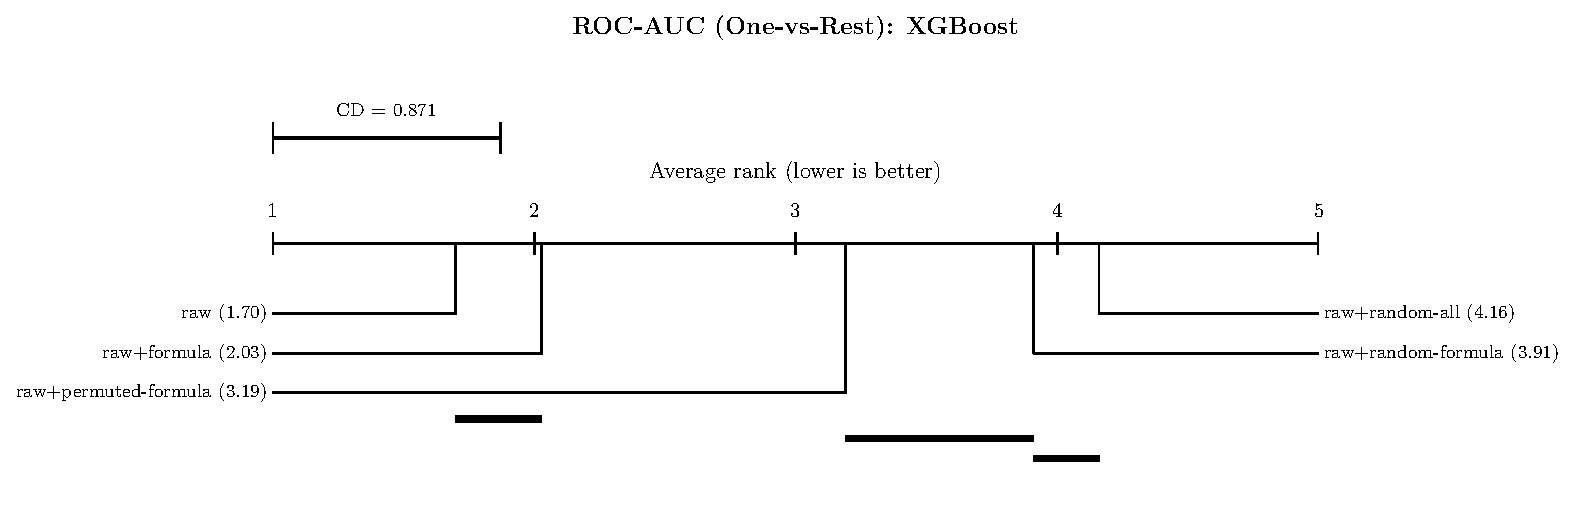
\includegraphics[width=0.85\linewidth]{figures/fig3b_cd_xgboost.pdf}
\caption{Critical-difference diagrams for ROC-AUC with logistic regression (top) and XGBoost (bottom) over the 49 datasets (Nemenyi test, $\alpha = 0.05$, $k = 5$, CD $= 0.87$; lower average rank is better). Formula features rank first for LR and second behind raw features for XGBoost; in both cases the permuted-formula and random controls are more than one critical difference behind the aligned formula matrix.}\label{fig:cd}
\end{figure}

\subsection*{Per-generator results}

Table~\ref{tab:generators} reports the semantic and direct contrasts for each generator separately, on the datasets it covers (48 for GPT-5.5 Pro, 44 for Gemini 3.1 Pro Preview, 40 for Claude Opus 4.7, 39 for Claude Sonnet 4.6).

\begin{table}[tbp]
\caption{Semantic control and direct effect by schema generator (linear/SVM schemas, ROC-AUC, one generator at a time on the datasets it covers). Columns as in Table~\ref{tab:semantic-direct}.}\label{tab:generators}
\centering
\small
\begin{adjustbox}{max width=\linewidth}
\begin{tabular}{llrrrrrrr}
\toprule
Generator & Downstream model & \(N\) & Semantic \(\Delta\) & W/L & \(p\) & Direct \(\Delta\) & W/L & \(p\) \\
\midrule
GPT-5.5 Pro & Logistic regression & 48 & +0.0150 & 46/1 & $<$0.001 & +0.0108 & 33/14 & $<$0.001 \\
 & KNN & 48 & +0.0520 & 44/4 & $<$0.001 & +0.0076 & 29/19 & 0.015 \\
 & Random forest & 48 & +0.0099 & 32/14 & 0.003 & +0.0026 & 20/26 & 0.931 \\
 & XGBoost & 48 & +0.0098 & 37/8 & $<$0.001 & +0.0009 & 21/24 & 0.929 \\
\midrule
Gemini 3.1 Pro Preview & Logistic regression & 44 & +0.0134 & 42/2 & $<$0.001 & +0.0081 & 33/11 & $<$0.001 \\
 & KNN & 44 & +0.0476 & 42/2 & $<$0.001 & +0.0052 & 22/22 & 0.154 \\
 & Random forest & 44 & +0.0083 & 26/17 & 0.026 & +0.0010 & 20/23 & 0.853 \\
 & XGBoost & 44 & +0.0081 & 33/10 & $<$0.001 & -0.0002 & 18/25 & 0.603 \\
\midrule
Claude Opus 4.7 & Logistic regression & 40 & +0.0193 & 37/2 & $<$0.001 & +0.0136 & 33/6 & $<$0.001 \\
 & KNN & 40 & +0.0548 & 40/0 & $<$0.001 & +0.0108 & 27/13 & 0.004 \\
 & Random forest & 40 & +0.0083 & 31/8 & $<$0.001 & +0.0013 & 17/22 & 0.961 \\
 & XGBoost & 40 & +0.0090 & 32/7 & $<$0.001 & -0.0002 & 15/24 & 0.225 \\
\midrule
Claude Sonnet 4.6 & Logistic regression & 39 & +0.0144 & 35/3 & $<$0.001 & +0.0098 & 33/5 & $<$0.001 \\
 & KNN & 39 & +0.0512 & 38/1 & $<$0.001 & +0.0068 & 28/11 & 0.006 \\
 & Random forest & 39 & +0.0095 & 29/9 & $<$0.001 & +0.0019 & 20/18 & 0.646 \\
 & XGBoost & 39 & +0.0065 & 34/4 & $<$0.001 & -0.0009 & 17/21 & 0.528 \\
\bottomrule
\end{tabular}
\end{adjustbox}
\end{table}

\subsection*{Classical baseline settings}

We ran three classical automated feature-engineering baselines on exactly the DASEF protocol: the same cap-then-split rows (the evaluation split is row-identical to the stored DASEF matrices, asserted at run time), the same 5\(\times\)2 CV, and the same four downstream models. The baselines are pairwise polynomial interactions (interaction-only products, top 12 selected by mutual information), OpenFE (top 12 generated features), and autofeat (one feature-engineering step with log, square-root, and square transforms). To mirror the LLM generator, which sees only a summary of the 30\% design split, each classical system is fitted on the design split (where it may use labels) and its features are then materialized on the evaluation split; no evaluation-split label is used outside the cross-validation training folds. This is stricter than the common practice of selecting features on the full evaluation data, and it leaves the classical systems only a few hundred design rows on the smallest datasets, a limitation of the matched protocol rather than of the systems. OpenFE was run in its first stage only, with two data blocks, at least 100 candidate features, one repeat, and seed 42, and its transform step sees the design and evaluation feature values (never labels) together because its group-by operators require both; the polynomial selector uses mutual information with random state 42; and the classical systems operate on a numeric encoding of the inputs (ordinal category codes and median imputation fitted on the design split), while the downstream models receive the raw columns plus the generated columns. Polynomial features cover all 49 datasets. OpenFE covers 47: it crashes natively on bng\_tic\_tac\_toe and mushroom (reproducibly, inside its own worker pool), and those two datasets are excluded from its rows. Autofeat returns additional features on 19 of the 49 datasets and is compared on those. On balanced accuracy OpenFE is ahead for KNN (\(+0.023\) versus \(+0.013\), \(p = 0.004\)) and RF (\(+0.012\) versus \(+0.008\), \(p = 0.016\)).

\subsection*{Post-cutoff replication: generation settings, knowledge cutoffs, and scope}

Schemas are generated only from each dataset's design split (a 20\% design split with no row cap, versus the 30\% split and 5,000-row cap of the main benchmark) using GPT-5.5 Pro and Gemini 3.1 Pro Preview; we evaluate the raw, formula, and random-control matrices, add the column-permuted formula control post hoc from the stored formula matrices (each generated column independently row-permuted, seed 42, evaluated with the same folds), and do not generate per-row judgments. Unlike the main benchmark, which uses the linear/SVM family only, the post-cutoff analysis uses all three schema families of both generators: the completed runs of a dataset (six, or five for prediction markets) are averaged per dataset before the Wilcoxon test, for the permuted, random-formula, and direct contrasts alike. The GPT-5.5 Pro distance-family cell on clinical trials required a second generation call after the first response failed JSON parsing. Four of the six repackage records that were publicly available before the model cutoffs (the underlying water-quality, hyperspectral, tracker, and clinical-trial data), so the control addresses memorization of these specific tables and of feature recipes published for them, not all prior exposure to the domains. Memorized formulas for these specific tables are not a plausible explanation of the effect here, because the tables did not exist in this form when the models were trained (OpenAI documents a 1 December 2025 knowledge cutoff for GPT-5.5 Pro\footnote{\url{https://developers.openai.com/api/docs/models/gpt-5.5-pro}, accessed 11 October 2026; the page lists \texttt{gpt-5.5-pro-2026-04-23} as the default snapshot.}; Google publishes no knowledge cutoff for Gemini 3.1 Pro Preview, but its public-preview release date of 19 February 2026 precedes the creation of all six tables\footnote{\url{https://ai.google.dev/gemini-api/docs/models/gemini-3.1-pro-preview} and \url{https://docs.cloud.google.com/vertex-ai/generative-ai/docs/models/gemini/3-1-pro}, accessed 11 October 2026.}). In Table~\ref{tab:postcutoff} the 5/1 semantic cells have \(p = 0.063\) for KNN ROC-AUC and RF balanced accuracy and \(p = 0.16\) for RF ROC-AUC, and all four models are positive in mean for both metrics. The weaker count-matched noise control (\texttt{raw+random-formula}) gives the same picture (ROC-AUC: LR \(+0.042\), RF \(+0.019\), KNN \(+0.084\), XGBoost \(+0.021\); 5/6 or 6/6 in every cell). The injected random-feature controls degrade KNN, RF, and XGBoost relative to raw features and leave LR roughly unchanged, so the gap is not a dimensionality artifact. With only six datasets these effects are a supportive replication rather than a powered confirmation; grouped cross-validation and redefined targets are future work.

\subsection*{Anonymized-column control: prompt contents, remaining cues, and like-for-like comparison}

Column names are replaced by generic tokens (\texttt{x001}, \texttt{x002}, \ldots), the dataset name and the target column name are replaced by generic tokens (the OpenML identifier is never part of a prompt), and the distributional summary (dtype, mean/std/min/max, missing rate, number of distinct values, category frequencies, row count, class balance) is retained. Two identifying cues remain: the class-label strings in the class-balance entry (such as \texttt{>50K}, \texttt{tested\_positive}, or \texttt{spam}) and, for credit-g, the categorical value strings, so the control removes column semantics rather than every cue to dataset identity. Like for like, the anonymized effect is not smaller than the same generator's named-column effect, so on these ten datasets column semantics add no measurable increment beyond the domain-agnostic component; the four-generator named-column average on the same ten datasets is similar (LR \(+0.012\), the mean of the core rows of Table~\ref{tab:per-dataset}), but that comparison mixes generators. The anonymized control uses a single generator, so it is a directional check rather than a full re-run of the multi-generator benchmark.

\subsection*{Random-expression control: limitations in detail}

The random-expression control draws five random schemas per cell from a fixed vocabulary with uniform template and column choices and averages their scores; a stronger label-free baseline, such as search over the same vocabulary with a validation criterion, might narrow the LLM-minus-random gap further, and the classical baselines of Section~\ref{sec:classical} are the label-using version of that comparison; its templates reference at most two columns, whereas many LLM formulas combine three or more, and LLM formula columns are clipped to the generator's declared range while random expressions use the design-split range.

\subsection*{Downstream-awareness diagnostic}

The pipeline included schema prompts targeted to model families such as linear/SVM, tree, and distance-based models. Across the core tier (10 datasets, 4 generators, 4 downstream models, 160 matched-versus-best-mismatched ROC-AUC comparisons on the raw-to-formula contrast), the matched prompt family beat the better of the two mismatched families in 57 comparisons and lost in 103 (44 of 120 when restricted to LR, RF, and KNN; 48 of 160 on balanced accuracy), consistent with chance (the expected win rate against the better of two alternatives under the null is one third). Model-family prompting does not reliably produce better-matched features in these experiments, which is also why the benchmark-wide analyses use a single family; a larger core tier may reveal family-specific effects.

